\section{Approach}
\label{sec:specapproach}
Our approach consists of five major components:
the framework reader, CSE, code downloader, code
analyzer, and spot builder. Figure~\ref{fig:architecture} shows an overview of all components
and flows among different components. We use JUnit
as an illustrative example for explaining our approach. 
\begin{figure}[t]
\centering
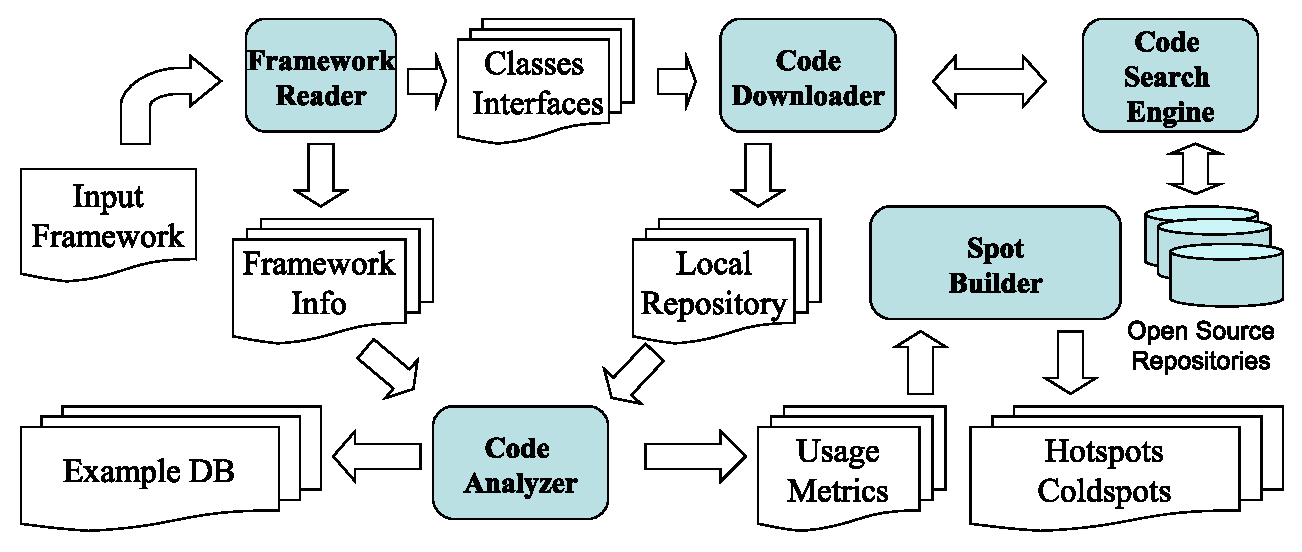
\includegraphics[scale=0.38,clip]{Framework_overview1.eps}
\caption{Overview of the SpotWeb approach} \label{fig:architecture}
\end{figure}
%--------------------------------------------------------------------------------
\subsection{Framework Reader} 
The framework reader component
takes a framework, say JUnit, as input and extracts the \emph{FrameworkInfo}
information. The \emph{FrameworkInfo} includes all classes, all interfaces, public
or protected methods of each class and interface.
%--------------------------------------------------------------------------------
\subsection{Code Downloader} 
The code downloader interacts with a CSE to download relevant code examples. 
For example, the code downloader constructs
a query such as ``\CodeIn{lang:java junit.framework.TestSuite}'' for
gathering relevant code examples of the \CodeIn{TestSuite} class.
The downloaded code examples, referred as \emph{LocalRepository}, are given as input
to the code analyzer. The code examples stored in the \emph{LocalRepository}
are often partial as CSE gathers individual source files,
instead of entire projects. \Fix{In our approach, we used Google code search~\cite{GCSE}
for gathering relevant code code examples. There are two main reasons
for using Google code search as an underlying search engine in our approach: Google code search
provides open APIs to interact through client code and is well-maintained.}

%--------------------------------------------------------------------------------
\subsection{Code Analyzer} 
The code analyzer analyzes code examples 
stored in the \emph{LocalRepository} statically and computes
\emph{UsageMetrics} for all classes, methods, exceptions, and constants of the input
framework. As these code examples are partial,
the code analyzer uses several type heuristics for resolving object types.
These type heuristics are described in our previous approach, called PARSEWeb~\cite{thummalapenta07:parseweb}.
The \emph{UsageMetrics} capture several ways of how often a class or an interface or a method 
of the input framework is used by gathered code examples.
The \emph{UsageMetrics} for a class include the
number of created instances (more precisely, the number of
constructor-call sites) and the number of times that the class is
extended. For an interface, the \emph{UsageMetrics} include the number
of times that the interface is implemented. We use notations
$IN_j$, $EX_j$, and $IM_j$ for the number of instances,
the number of extensions, and the number of implementations, respectively.
The consolidated usage metric $UM_j$ for a class or an interface 
is the sum of all the three preceding metrics. The \emph{UsageMetrics}
for an exception class include the number of times that the exception class
is used in the \CodeIn{catch} blocks or the \CodeIn{throw} statements. 

The code analyzer computes three types of \emph{UsageMetrics} for
methods: Invocations, Overrides, and Implements.
The \emph{Invocations} metric gives the number of times that the
method is invoked by the code examples. The \emph{Overrides} metric
gives the number of times that the method is overridden by the code
examples to define a new behavior. The \emph{Implements} metric,
specific for interfaces, gives the number of times that the method
is implemented. \Fix{The code analyzer considers \CodeIn{static} methods as regular methods.} 
For constructors, the code analyzer computes only the \emph{Invocations} metric. 
We use notations $IN_i$, $OV_i$, and $IM_i$
for invocations, overrides, and implementations, respectively. 
The overall usage metric ($UM_i$) for a method is the sum of all the three
preceding metrics. 

The code analyzer identifies constants defined by the input framework through
the Java keywords such as \CodeIn{final} and \CodeIn{static}. The \emph{UsageMetrics}
for such a constant include the number of times that the constant is referred
by code examples gathered from CSE.

The code analyzer also gathers code examples for each class or method and 
stores these code examples in a repository, referred as \CodeIn{ExampleDB}. The \CodeIn{ExampleDB} is used
for recommending relevant code examples for a class or a method requested by the user. The relevant
code examples can further assist users in making an effective reuse of API classes and methods of the
input framework. 

\begin{figure}[t]
\begin{CodeOut}
Input: UsageMetrics of classes and methods, HT percentage\\
Output: Hotspot hierarchies and their dependencies\\
1:\emph{SortedMET} = Sort methods based on their usage metric values;\\
2:foreach \emph{$MET_i$} in $SortedMET$ \{\\
\hspace*{0.3in}if ($UM_i$ $\neq$ 0) \\
\hspace*{0.5in}if (Position of $MET_i$ $\leq$ ($HT$ * Size of $SortedMET$))\\
\hspace*{0.8in}Set $MET_i$ type as $HOTSPOT$; \\
%\hspace*{0.5in}else \\
%\hspace*{0.8in}Set $MET_i$ type as $WEAKSPOT$;\\ 
\hspace*{0.2in}\}\\
3:\{$C_1$, ... $C_n$\} = Group $HOTSPOT$ $MET_i$ based on their \\\hspace*{0.2in}declaring classes;\\
//Assign ranks to each $C_i$ and classify into templates and hooks\\
4:foreach \emph{$C_i$} in \{$C_1$, ... $C_n$\} \{\\
\hspace*{0.3in}Rank of $C_i$ = Minimum rank among all $MET_i$ of the $C_i$;\\
\hspace*{0.3in}if $C_i$ is an \emph{Interface} or \emph{Abstract class} or ($EX_i$ $>$ $IN_i$)\\
\hspace*{0.5in}Set type of $C_i$ to $HOOK$;\\
\hspace*{0.3in}otherwise\\ 
\hspace*{0.5in}Set type of $C_i$ to $TEMPLATE$;\\
\hspace*{0.2in}\}\\
5:Group $C_i$ of the same type into hierarchies based on inheritance;\\
6:Associate hook hierarchies to template hierarchies;\\
7:Define dependencies between template hierarchies;\\
8:Output hook and template hierarchies as hotspot hierarchies;\\
\end{CodeOut}
\caption{\small{Algorithm used for detecting hotspots through computed
\emph{UsageMetrics}}} \label{alg:hotspotalgo}
\end{figure}
%---------------------------------------------------------------------------------
\subsection{Spot Builder} 
The spot builder component (SBC) analyzes gathered code examples and detects 
hotspots and coldspots.
%---------------------------------------------------------------------------------
\subsubsection{Identification of hotspots}
The spot builder component (SBC) uses computed \emph{UsageMetrics} for
detecting hotspots. The algorithm used by SBC for detecting hotspots
is shown in Figure~\ref{alg:hotspotalgo}. We next describe the algorithm 
through an illustrative example shown in Figure~\ref{fig:frameworkex}. The figure
shows four classes $C_1$, $C_2$, $C_3$, and \CodeIn{ExceptClass}, and their declarations. 
The class $C_3$ is an \CodeIn{abstract} class. The \CodeIn{ExceptClass}
is an \CodeIn{Exception} class that can appear in exception-handling
constructs such as \CodeIn{catch} blocks. The figure also shows
computed usage metrics for each class, and its methods and constant variables. For example,
the class $C_1$ is instantiated for 10 times (shown as \CodeIn{IN}=10)
and the abstract class $C_3$ is extended for 12 times (shown as \CodeIn{EX}=12). 
The method $m_{2\_1}$ is invoked for 6 times and is overridden for 2 times.
Similarly, the constant \CodeIn{constC1} is accessed 6 times and the 
exception class \CodeIn{ExceptClass} is detected in \CodeIn{catch} blocks
for 9 times among gathered code examples.

\begin{figure}[t]
\centering
\includegraphics[scale=0.43,clip]{figs/Approach_Example1.eps}
\caption{Example classes of a sample framework} \label{fig:frameworkex}
\end{figure}

Initially, SBC sorts $UM$ values of all methods, constants, and
exception classes. 
SBC uses a threshold percentage (referred as $HT$) and selects the
top $HT$ methods, whose usage metric is non-zero, as hotspot methods. For example, for a $HT$ of 45\%,
SBC identifies the methods such as $m_{3\_1}$, $m_{3\_2}$, $m_{3\_3}$, and $c_1$ as hotspot
methods. SBC groups the hotspot methods based on their declaring classes. 
The resulting classes are sorted based on the minimum rank among included hotspot methods in each class.
In the current example, the grouping process results in 
classes $C_3$ (methods: $m_{3\_1}$, $m_{3\_2}$, and $m_{3\_3}$), 
$C_1$ (methods: $c_1$ and $m_{1\_1}$), and $C_2$ (methods: $c_2$ and $m_{2\_1}$).
After grouping, SBC uses computed metrics of classes
to classify these classes further into templates and hooks. The criteria
used for classifying hotspot classes into templates and hooks are shown in Step 4 of the algorithm.
For the current example, SBC identifies class $C_3$ as a \CodeIn{HOOK} class, and classes
$C_1$ and $C_2$ as \CodeIn{TEMPLATE} classes. SBC further 
groups the classes of the same category based on their inheritance relationship. For example,
if $C_1$ has a parent class $P_1$ and both classes are classified as \CodeIn{TEMPLATE} classes,
SBC groups $C_1$ and $P_1$ into the same hierarchy.

SBC identifies dependencies among the detected hotspot hierarchies based on arguments
passed to methods of those classes. For example, if a template class, say X, has a constructor that requires
an instance of another template class, say Y, then SpotWeb captures
dependency of the form ``X $\rightarrow$ Y'', which describes that X
requires Y. SBC identifies two kinds of dependencies: \CodeIn{TEMPLATE\_HOOK}
and \CodeIn{TEMPLATE\_TEMPLATE}. A \CodeIn{TEMPLATE\_HOOK} dependency defines a relationship
between a template hierarchy and a hook hierarchy. SBC identifies that
a template hierarchy is dependent on a hook hierarchy if methods in the template
hierarchy types include some classes in the hook hierarchy as arguments. Such a dependency describes
that the users have to first define a new behavior for those related hook classes, say
extend the classes, and use the instances of those classes
as arguments. For example, SBC identifies that the class $C_1$ has a 
\CodeIn{TEMPLATE\_HOOK} dependency with 
the class $C_3$ as the method \CodeIn{$m_{1\_1}$} requires an instance of $C_3$ 
as an argument. Similarly, SBC identifies \CodeIn{TEMPLATE\_TEMPLATE}
hierarchies when one template hierarchy is dependent on another template hierarchy.
For example, the class $C_2$ has a \CodeIn{TEMPLATE\_TEMPLATE} dependency
with the class $C_1$. 

\Comment{
\begin{figure}[t]
\begin{CodeOut}
Input: A method $M_i$ of a class $C_j$\\
Output: Is the method a coldspot or not?\\
if ($UM_i$ $\neq$ 0) Return false;\\
if ($C_j$ is an interface) \{\\
\hspace*{0.3in}//verify all implemented methods of $M_i$\\
\hspace*{0.3in}if (All implemented methods of $M_i$ are coldspots) 
\hspace*{0.5in}Return true; \\
\hspace*{0.3in}else \\
\hspace*{0.5in}Return false; \}\\
if ($M_i$ is abstract) \{\\
\hspace*{0.3in}//Verify all overridden methods of $M_i$\\
\hspace*{0.3in}if (All overridden methods of $M_i$ are coldspots) 
\hspace*{0.5in}Return true; \\
\hspace*{0.3in}else \\
\hspace*{0.5in}Return false; \}\\
if (All callers of $M_i$ are coldspots) \\
\hspace*{0.3in}Return true; \\
else \\
\hspace*{0.3in}Return false;
\end{CodeOut}
\caption{\label{alg:coldspotalg}Algorithm for detecting whether a method is a coldspot.} 
\end{figure}}
\begin{figure}[t]
\begin{CodeOut}
Input: A method $M_i$ of a class $C_j$\\
Output: Is the method a coldspot or not?\\
1:Return false if the method is reused atleast once;\\
2:if $C_j$ is an interface \\
%\hspace*{0.3in}//verify all implemented methods of $M_i$\\
\hspace*{0.3in}Return true if all implemented methods of $M_i$ are coldspots; 
\hspace*{0.3in}Otherwise return false; \\
3:if $M_i$ is abstract \\
%\hspace*{0.3in}//Verify all overridden methods of $M_i$\\
\hspace*{0.3in}Return true if all overridden methods of $M_i$ are coldspots;
\hspace*{0.3in}Otherwise return false; \\
4:Return true if all callers of $M_i$ are coldspots \\
\hspace*{0.3in}Otherwise return false; \\
\end{CodeOut}
\caption{\label{alg:coldspotalg}Algorithm for detecting whether a method is a coldspot.} 
\end{figure}
%--------------------------------------------------------------------------
\subsubsection{Identification of coldspots}
SBC identifies classes and methods of the input framework that are rarely or never used
by gathered code examples as coldspots. However, detecting coldspots based on only the
\emph{UsageMetrics} can give many false positives. For example, the
\emph{UsageMetrics} for an abstract method defined in a class can be zero, as
gathered code examples refer to the concrete implementation provided
by some of the abstract classes's subclasses. In this case, this abstract method is
not a coldspot as the method is indirectly referenced through the
subclasses. Therefore, to reduce the number of false positives
while identifying coldspots, the code analyzer uses a recursive
algorithm shown in Figure~\ref{alg:coldspotalg}. 
\Comment{The \emph{UsageMetrics} referred by the algorithm is the sum of metrics
\emph{Invocations}, \emph{Overrides}, and \emph{Implements} computed
for a method. If computed \emph{UsageMetrics} are not zero, then
the method is identified not as a coldspot. If the current method
belongs to an interface, our algorithm recursively checks whether
all the corresponding methods in the implemented classes of the
input framework are also coldspots. If all of them are coldspots, the
code analyzer identifies the current method as a coldspot. The code
analyzer uses a similar approach when the method is abstract. If the
current method under analysis does not belong to any of the
preceding categories, the code analyzer checks whether all other
methods of the input framework that invoke the current method are also
coldspots.} Step 4 of the algorithm (related to callers)
is performed to identify indirect usages of a method of the input framework. 
SBC groups detected coldspot methods into their declaring classes.

We developed SpotWeb as an Eclipse plugin. SpotWeb can be invoked by selecting
a menu item available on projects in Eclipse. In the SpotWeb implementation, 
we used the $HT$ percentage of 15\%, which is derived based on our
initial empirical experience.